% !TEX root=./adl.tex

\section{Using LLMs: Prompting, Tools, RAG and Agents}

% =======================================================================
\subsection{From Chat Completion to Agentic Systems}

% -----------------------------------------------------------------------
\begin{frame}{Motivation: LLMs as Building Blocks}

  Pretrained + instruction-tuned LLMs~\cite{ouyang2022instructgpt} are powerful general-purpose
  text predictors, but on their own they suffer from well-known limitations:

  \vspace{0.3em}
  \begin{description}
    \item[Knowledge cutoff] Training data is frozen; cannot answer questions about recent events.
    \item[Hallucination] Confidently produce wrong facts when knowledge is missing.
    \item[No grounding] Cannot access private documents, databases, files, or the user's machine.
    \item[Closed world] Cannot perform actions: send mails, run code, query APIs, control a browser.
    \item[Limited reasoning] Single forward pass is not enough for problems that require search or backtracking.
  \end{description}

  \vspace{0.5em}
  \textbf{Key idea of \emphdef{agentic AI}:} treat the LLM as a \emph{component} inside a larger
  system that augments it with
  \begin{itemize}[nosep]
    \item structured \textbf{prompts} and \textbf{in-context examples} (steer behavior)
    \item \textbf{chain-of-thought} (use extra tokens for reasoning)
    \item \textbf{tools} (read files, call APIs, execute code)
    \item \textbf{retrieval} (inject relevant knowledge into context)
    \item \textbf{memory} (state that persists across turns)
    \item a \textbf{control loop} (decide when to stop)
  \end{itemize}
\end{frame}

% -----------------------------------------------------------------------
\begin{frame}{Spectrum: From Single Call to Autonomous Agent}

  \begin{center}
    \begin{tikzpicture}[
      scale=0.85, every node/.style={scale=0.85},
      stage/.style={draw, rounded corners, minimum width=2.6cm, minimum height=1.2cm,
                    align=center, font=\scriptsize},
      arr/.style={-Stealth, thick},
    ]
      \node[stage, fill=blue!8]   (s1) at (0,0)  {\textbf{Prompt}\\(zero/few-shot)};
      \node[stage, fill=blue!12]  (s2) at (3,0)  {\textbf{+ CoT}\\reason in tokens};
      \node[stage, fill=blue!18]  (s3) at (6,0)  {\textbf{+ Retrieval}\\ground in docs};
      \node[stage, fill=blue!25]  (s4) at (9,0)  {\textbf{+ Tools}\\act on world};
      \node[stage, fill=blue!35]  (s5) at (12,0) {\textbf{Agent loop}\\plan, act, observe};

      \draw[arr] (s1) -- (s2);
      \draw[arr] (s2) -- (s3);
      \draw[arr] (s3) -- (s4);
      \draw[arr] (s4) -- (s5);

      \node[font=\scriptsize, gray] at (6, -1.2)
        {fixed control flow $\longrightarrow$ LLM-driven control flow};
    \end{tikzpicture}
  \end{center}

  \vspace{0.5em}
  \begin{block}{Workflows vs.\ Agents \cite{anthropic2024agents}}
    \begin{description}
      \item[Workflow] Pre-defined chain of LLM calls and tool calls. Predictable, debuggable, cheap. Use when the task decomposes into known steps.
      \item[Agent] LLM \emph{itself} decides at each step whether to call a tool, retrieve, reflect, or answer. Flexible but expensive and harder to control. Use only when the path is not knowable up-front.
    \end{description}
  \end{block}

  \textbf{Rule of thumb:} start with the simplest pattern that works. Add complexity only when measurably needed.
\end{frame}

% =======================================================================
\subsection{Prompting}

% -----------------------------------------------------------------------
\begin{frame}{Anatomy of a Chat Prompt}

  Modern instruction-tuned LLMs expect input as a sequence of \emphdef{role-tagged messages}.
  Roles are baked into the chat template at fine-tuning time.

  \vspace{0.3em}
  \begin{columns}
    \begin{column}{0.52\textwidth}
      \begin{center}
        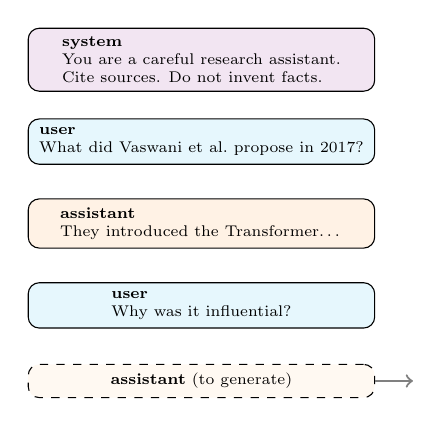
\begin{tikzpicture}[
          scale=0.8, every node/.style={scale=0.8},
          msg/.style={draw, rounded corners, minimum width=5.5cm, align=left,
                      font=\scriptsize, inner sep=4pt},
        ]
          \node[msg, fill=violet!10] (sys) at (0,3)
            {\textbf{system}\\
             You are a careful research assistant.\\
             Cite sources. Do not invent facts.};
          \node[msg, fill=cyan!10] (usr) at (0,1.7)
            {\textbf{user}\\
             What did Vaswani et al.\ propose in 2017?};
          \node[msg, fill=orange!10] (asst) at (0,0.4)
            {\textbf{assistant}\\
             They introduced the Transformer\ldots};
          \node[msg, fill=cyan!10] (usr2) at (0,-0.9)
            {\textbf{user}\\
             Why was it influential?};
          \node[msg, dashed, fill=orange!5] (cont) at (0,-2.1)
            {\textbf{assistant} (to generate)};
          \draw[->, thick, gray] (cont.east) -- ++(0.6,0);
        \end{tikzpicture}
      \end{center}
    \end{column}
    \begin{column}{0.46\textwidth}
      \textbf{Role conventions:}
      \begin{description}[style=nextline]
        \item[\texttt{system}] Persistent instructions, persona, output format, safety rules. Set once.
        \item[\texttt{user}] The request to answer.
        \item[\texttt{assistant}] Previous model responses (multi-turn history).
        \item[\texttt{tool}] Result of a tool call (see later).
      \end{description}

      \vspace{0.3em}
      \textbf{Under the hood} the chat template flattens these into a single token stream
      with special tokens like \texttt{<|im\_start|>}, \texttt{<|im\_end|>}.
      \emph{The model has no notion of ``role'' beyond what those tokens mean.}
    \end{column}
  \end{columns}
\end{frame}

% -----------------------------------------------------------------------
\begin{frame}{Prompt Engineering: Practical Principles}

  Prompting is the cheapest way to steer behavior: no training, no data, instant feedback.
  A few rules consistently help.

  \vspace{0.3em}
  \begin{description}
    \item[Be specific and concrete] State the task, the input, the desired output format,
      and any constraints explicitly. ``Summarize'' is ambiguous; ``summarize in 3 bullets,
      $\le 15$ words each'' is not.
    \item[Show, don't tell] Add 1--5 worked examples (\emph{few-shot}) when the task is
      hard to describe but easy to demonstrate (formatting, style, edge cases).
    \item[Decompose] Break a hard task into named sub-steps. Either chain calls
      (workflow) or ask the model to follow the steps in one go.
    \item[Give the model an out] Allow ``I don't know'' / ``insufficient information'' as a
      valid answer to reduce hallucination.
    \item[Constrain the output] Request JSON, XML tags, or a specific schema when the
      output will be parsed by code. Many APIs support \emph{structured output}
      / grammar-constrained decoding.
    \item[Put important things at the boundaries] Models attend most to the start and
      end of the context (positional bias, ``lost in the middle''). Place key
      instructions in the system prompt and the question last.
    \item[Iterate with evals] Treat prompts like code: keep them under version control
      and measure changes against a small held-out set of inputs.
  \end{description}
\end{frame}

% =======================================================================
\subsection{In-Context Learning}

% -----------------------------------------------------------------------
\begin{frame}[fragile]{In-Context Learning (Few-Shot Prompting)}

  \cite{brown2020gpt3} showed that sufficiently large LMs can learn new tasks from
  a handful of examples placed \emph{in the prompt}, with no weight updates.
  This is called \emphdef{in-context learning} (ICL).

  \vspace{0.3em}
  \begin{columns}
    \begin{column}{0.52\textwidth}
      \textbf{Three regimes:}
      \begin{description}
        \item[Zero-shot] Just a task description.
        \item[One-shot] Description $+$ 1 example.
        \item[Few-shot] Description $+$ $k$ examples ($k \approx 2\text{--}32$).
      \end{description}

      \vspace{0.3em}
      \textbf{When to use ICL:}
      \begin{itemize}[nosep]
        \item Task is hard to specify in words but easy to demonstrate.
        \item You need a specific output format.
        \item You have $<\!\!100$ labeled examples (otherwise consider fine-tuning).
        \item Task distribution is small enough to fit in the context window.
      \end{itemize}

      \vspace{0.3em}
      \textbf{Practical tips:}
      \begin{itemize}[nosep]
        \item Use \emph{diverse} examples covering edge cases.
        \item Order matters: recent examples have more influence (recency bias).
        \item Class balance matters for classification ICL.
      \end{itemize}
    \end{column}
    \begin{column}{0.46\textwidth}
      {\scriptsize\textbf{Few-shot example: sentiment}}
\begin{lstlisting}[basicstyle=\scriptsize\ttfamily, frame=single, backgroundcolor=\color{blue!4}, rulecolor=\color{blue!40!black}, keywordstyle={}, commentstyle={}, stringstyle={}, xleftmargin=0.3em, xrightmargin=0.3em, mathescape=false]
Classify the sentiment as
positive, negative or neutral.

Review: "Loved every minute."
Sentiment: positive

Review: "It was fine, I guess."
Sentiment: neutral

Review: "Total waste of money."
Sentiment: negative

Review: "Best purchase this year!"
Sentiment:
\end{lstlisting}
      \vspace{0.2em}
      {\scriptsize The model continues with \texttt{positive}, having induced both the format and the label set.}
    \end{column}
  \end{columns}
\end{frame}

% =======================================================================
\subsection{Chain of Thought}

% -----------------------------------------------------------------------
\begin{frame}[fragile]{Chain-of-Thought (CoT) Prompting}

  \cite{wei2022cot}: For multi-step problems, asking the model to ``think step by step''
  before answering dramatically improves accuracy on arithmetic, commonsense, and symbolic
  reasoning benchmarks.

  \vspace{0.3em}
  \begin{columns}
    \begin{column}{0.5\textwidth}
      {\scriptsize\textbf{Standard prompting}}
\begin{lstlisting}[basicstyle=\scriptsize\ttfamily, frame=single, backgroundcolor=\color{red!4}, rulecolor=\color{red!50!black}, keywordstyle={}, commentstyle={}, stringstyle={}, xleftmargin=0.3em, xrightmargin=0.3em, mathescape=false]
Q: Roger has 5 balls. He buys
2 cans of 3. How many now?
A: 11
Q: A cafeteria had 23 apples,
used 20, bought 6 more. How many?
A: ???
\end{lstlisting}
    \end{column}
    \begin{column}{0.5\textwidth}
      {\scriptsize\textbf{Chain-of-thought prompting}}
\begin{lstlisting}[basicstyle=\scriptsize\ttfamily, frame=single, backgroundcolor=\color{green!4}, rulecolor=\color{green!40!black}, keywordstyle={}, commentstyle={}, stringstyle={}, xleftmargin=0.3em, xrightmargin=0.3em, mathescape=false]
Q: Roger has 5 balls. He buys
2 cans of 3. How many now?
A: He had 5. 2 cans * 3 = 6.
   5 + 6 = 11. Answer: 11.
Q: A cafeteria had 23 apples,
used 20, bought 6 more. How many?
A: ???
\end{lstlisting}
    \end{column}
  \end{columns}

  \vspace{0.4em}
  \textbf{Why does it work?}
  \begin{itemize}[nosep]
    \item A single forward pass has fixed compute per token. Letting the model emit
      \emph{intermediate tokens} effectively gives it more compute to ``think''.
    \item Intermediate steps act as a working memory written into the context.
    \item Each step conditions the next: the joint distribution over (rationale, answer) is easier to model than the answer alone.
  \end{itemize}

  \vspace{0.3em}
  \textbf{Zero-shot CoT}~\cite{kojima2022zerocot}: simply appending ``\emph{Let's think step by step.}''
  to the prompt unlocks much of the gain without any examples.
  Modern reasoning-tuned models (o1, R1) emit long internal CoTs by default.
\end{frame}

% -----------------------------------------------------------------------
\begin{frame}{Beyond Linear CoT: Self-Consistency and Tree of Thoughts}

  \begin{columns}[T]
    \begin{column}{0.5\textwidth}
      \textbf{Self-consistency}~\cite{wang2023selfconsistency}
      \begin{itemize}[nosep]
        \item Sample $N$ different CoTs for the same question (temperature $> 0$).
        \item Extract the final answer from each.
        \item \emphdef{Majority vote} over answers.
      \end{itemize}
      \vspace{0.2em}
      Trades $N{\times}$ compute for substantially higher accuracy on tasks with a unique
      verifiable answer. The right reasoning path tends to converge on the same answer from many starts.
    \end{column}
    \begin{column}{0.5\textwidth}
      \textbf{Tree of Thoughts}~\cite{yao2023tot}
      \begin{itemize}[nosep]
        \item Treat reasoning as \emph{search over a tree} of partial thoughts.
        \item At each node, the LLM \emph{proposes} several next steps and \emph{evaluates} how promising each is.
        \item Use BFS/DFS with backtracking and pruning.
      \end{itemize}
      Useful for puzzles (Game of 24, crosswords) where one wrong step is fatal and exploration matters.
    \end{column}
  \end{columns}

  \vspace{0.5em}
  \begin{center}
    \begin{tikzpicture}[
      scale=0.75, every node/.style={scale=0.75},
      n/.style={draw, circle, inner sep=1.5pt, fill=blue!10, font=\tiny},
      good/.style={draw, circle, inner sep=1.5pt, fill=green!25, font=\tiny},
      bad/.style={draw, circle, inner sep=1.5pt, fill=red!15, font=\tiny},
      arr/.style={-Stealth},
    ]
      % Self-consistency
      \node[font=\scriptsize, anchor=west] at (-7.5, 2.4) {\textbf{Self-consistency}};
      \node[font=\tiny] (q) at (-5.5, 2.0) {Q};
      \foreach \i/\x in {1/-7.0, 2/-6.0, 3/-5.0, 4/-4.0} {
        \node[n] (a\i) at (\x, 0.8) {};
        \draw[arr] (q) -- (a\i);
      }
      \node[font=\tiny] at (-7.0, 0.2) {7};
      \node[font=\tiny] at (-6.0, 0.2) {7};
      \node[font=\tiny] at (-5.0, 0.2) {3};
      \node[font=\tiny] at (-4.0, 0.2) {7};
      \node[font=\tiny, green!50!black] at (-5.5, -0.6) {majority $\to$ 7};

      % Tree of thoughts
      \node[font=\scriptsize, anchor=west] at (1.0, 2.4) {\textbf{Tree of Thoughts}};
      \node[n] (r) at (4.0, 2.0) {};
      \node[good] (l1) at (2.5, 0.9) {};
      \node[bad]  (l2) at (4.0, 0.9) {};
      \node[n]    (l3) at (5.5, 0.9) {};
      \node[good] (m1) at (1.8, -0.2) {};
      \node[n]    (m2) at (3.0, -0.2) {};
      \node[n]    (m3) at (5.0, -0.2) {};
      \node[bad]  (m4) at (6.0, -0.2) {};
      \draw[arr] (r) -- (l1); \draw[arr] (r) -- (l2); \draw[arr] (r) -- (l3);
      \draw[arr] (l1) -- (m1); \draw[arr] (l1) -- (m2);
      \draw[arr] (l3) -- (m3); \draw[arr] (l3) -- (m4);
      \node[font=\tiny, green!50!black, anchor=west] at (6.5, 1.5) {expand};
      \node[font=\tiny, red!60!black,   anchor=west] at (6.5, 1.0) {prune};
    \end{tikzpicture}
  \end{center}
\end{frame}

% =======================================================================
\subsection{Tool Use}

% -----------------------------------------------------------------------
\begin{frame}{Tool Use: Letting the Model Act}

  \textbf{Why tools?} A pretrained LLM cannot
  \begin{itemize}[nosep]
    \item compute \texttt{17389 * 23491} reliably
    \item know today's weather, stock price, or git log
    \item read a file on the user's disk or query a database
    \item run unit tests or execute Python
  \end{itemize}
  Yet all of these are easy for tiny pieces of conventional code. \emphdef{Tool use}
  bridges the LLM and that code.

  \vspace{0.4em}
  \textbf{The protocol} (function calling, used by Claude, GPT, Gemini, \ldots
  \cite{anthropic2024toolUse}):
  \begin{enumerate}[nosep]
    \item Developer registers a list of \emph{tools}: name, natural-language description, JSON schema for arguments.
    \item The schemas are inserted into the prompt (typically the system message).
    \item When the model wants to call a tool, it emits a structured \texttt{tool\_use} block instead of a normal answer.
    \item The runtime parses the block, executes the tool, and appends the result as a \texttt{tool\_result} message.
    \item The model is invoked again with the augmented conversation and either calls more tools or produces a final answer.
  \end{enumerate}

  \vspace{0.3em}
  \cite{schick2023toolformer} \textbf{Toolformer}: train the model itself to insert API calls
  into its outputs by self-supervised data augmentation. Modern models are RL-fine-tuned
  on tool-use trajectories.
\end{frame}

% -----------------------------------------------------------------------
\begin{frame}{Tool Calling: Sequence Diagram}

  \begin{center}
    \begin{tikzpicture}[
      scale=0.85, every node/.style={scale=0.85},
      actor/.style={draw, rounded corners, fill=blue!10, minimum width=2.0cm, minimum height=0.55cm, font=\small},
      arr/.style={-Stealth, thick},
      msg/.style={font=\scriptsize, midway, fill=white, inner sep=1pt},
    ]
      \node[actor] (user)    at (-4.5, 4) {User};
      \node[actor] (runtime) at (-1.0, 4) {Runtime};
      \node[actor] (llm)     at ( 2.5, 4) {LLM};
      \node[actor] (tool)    at ( 6.0, 4) {Tool / API};

      \foreach \x in {-4.5, -1.0, 2.5, 6.0} {
        \draw[gray, dashed] (\x, 3.7) -- (\x, -3.0);
      }

      \draw[arr] (-4.5, 3.3) -- node[msg] {``weather in Paris?''} (-1.0, 3.3);
      \draw[arr] (-1.0, 2.7) -- node[msg] {prompt + tool schemas} (2.5, 2.7);
      \draw[arr] (2.5, 2.1)  -- node[msg, text=violet] {\texttt{tool\_use(get\_weather, \{city:Paris\})}} (-1.0, 2.1);
      \draw[arr] (-1.0, 1.5) -- node[msg] {HTTP call} (6.0, 1.5);
      \draw[arr] (6.0, 0.9)  -- node[msg] {\{temp:14, rain:0\}} (-1.0, 0.9);
      \draw[arr] (-1.0, 0.3) -- node[msg, text=violet] {\texttt{tool\_result(\ldots)}} (2.5, 0.3);
      \draw[arr] (2.5, -0.3) -- node[msg] {``It's 14$^\circ$C and dry.''} (-1.0, -0.3);
      \draw[arr] (-1.0, -0.9) -- node[msg] {final answer} (-4.5, -0.9);

      \node[font=\scriptsize, gray, align=left, anchor=west] at (-4.5, -2.0)
        {The model never touches the network itself: it only \emph{requests} a call.\\
         The runtime is the trust boundary. Tool calls can be sandboxed, rate-limited, audited.};
    \end{tikzpicture}
  \end{center}
\end{frame}

% =======================================================================
\subsection{Retrieval-Augmented Generation (RAG)}

% -----------------------------------------------------------------------
\begin{frame}{Retrieval-Augmented Generation: Why and What}

  \cite{lewis2020rag}: Combine a parametric LM with a non-parametric \emph{external memory}
  (a corpus of documents). At inference, retrieve relevant passages and feed them into
  the prompt as context.

  \vspace{0.3em}
  \textbf{What problems does it solve?}
  \begin{description}
    \item[Knowledge cutoff] Update the corpus, not the weights.
    \item[Private data] Index company docs, codebases, mails, that the base model has never seen.
    \item[Hallucination] Conditioning on retrieved text reduces fabrication when prompted to ``answer only from the sources''.
    \item[Citation] You can show the user \emph{which document} the answer came from.
    \item[Cost] Smaller models with retrieval can match larger models without it on knowledge-intensive tasks.
  \end{description}

  \vspace{0.4em}
  \textbf{Two paradigms.}
  \begin{description}
    \item[Closed-book] Model relies only on its weights. (Standard chat.)
    \item[Open-book / RAG] Prompt = \texttt{<system>} + \texttt{<retrieved chunks>} + \texttt{<question>}. Model is told to answer using the chunks.
  \end{description}
  See \cite{gao2023ragsurvey} for an extensive survey.
\end{frame}

% -----------------------------------------------------------------------
\begin{frame}{The RAG Pipeline}

  \begin{center}
    \begin{tikzpicture}[
      scale=0.78, every node/.style={scale=0.78},
      box/.style={draw, rounded corners, minimum height=0.7cm, align=center, font=\scriptsize},
      offline/.style={box, fill=orange!12},
      online/.style={box, fill=blue!12},
      arr/.style={-Stealth, thick},
    ]
      % --- Offline indexing (top row) ---
      \node[font=\scriptsize, anchor=west, text=orange!70!black] at (-7.5, 3.6) {\textbf{Offline: build the index}};
      \node[offline, minimum width=1.6cm] (docs) at (-6.0, 2.5) {Docs\\(PDF, MD, code)};
      \node[offline, minimum width=1.6cm] (chunk) at (-3.5, 2.5) {Chunk\\($\sim$200--800 tok)};
      \node[offline, minimum width=1.6cm] (embed) at (-1.0, 2.5) {Embed\\(encoder)};
      \node[offline, minimum width=1.6cm] (vdb)   at ( 1.7, 2.5) {Vector DB\\(ANN index)};
      \draw[arr] (docs)  -- (chunk);
      \draw[arr] (chunk) -- (embed);
      \draw[arr] (embed) -- (vdb);

      % --- Online query (bottom row) ---
      \node[font=\scriptsize, anchor=west, text=blue!70!black] at (-7.5, 1.0) {\textbf{Online: answer a query}};
      \node[online, minimum width=1.4cm] (q)   at (-6.0, -0.2) {Query};
      \node[online, minimum width=1.4cm] (qe)  at (-3.7, -0.2) {Embed};
      \node[online, minimum width=1.4cm] (sea) at (-1.4, -0.2) {Top-$k$ search};
      \node[online, minimum width=1.4cm] (rer) at ( 1.0, -0.2) {Rerank\\(opt.)};
      \node[online, minimum width=1.6cm] (prm) at ( 3.5, -0.2) {Build prompt\\(Q + chunks)};
      \node[online, minimum width=1.4cm] (llm) at ( 6.0, -0.2) {LLM};
      \node[online, minimum width=1.4cm, fill=green!18] (ans) at ( 8.2, -0.2) {Answer\\+ citations};
      \draw[arr] (q)   -- (qe);
      \draw[arr] (qe)  -- (sea);
      \draw[arr] (sea) -- (rer);
      \draw[arr] (rer) -- (prm);
      \draw[arr] (prm) -- (llm);
      \draw[arr] (llm) -- (ans);

      % --- Cross arrow from index ---
      \draw[arr, dashed, gray] (vdb.south) -- ++(0,-0.4) -| (sea.north);
    \end{tikzpicture}
  \end{center}

  \vspace{0.4em}
  \textbf{Two stages, two distinct concerns.}
  \begin{description}
    \item[Indexing (offline, batch)] chunking strategy, embedding model
      choice, metadata to keep alongside vectors. Done once per corpus.
    \item[Querying (online, latency-sensitive)] embedding the query, ANN
      search (FAISS, HNSW), optional reranking, prompt assembly, generation.
  \end{description}
\end{frame}

% -----------------------------------------------------------------------
\begin{frame}{Practical RAG: Pitfalls and Tricks}

  \textbf{Embeddings and retrieval}
  \begin{itemize}[nosep]
    \item \emphdef{Dense retrieval}~\cite{karpukhin2020dpr}: encode query and passage
      with the same model, take cosine similarity. Captures semantic similarity.
    \item \emphdef{Sparse retrieval} (BM25): keyword overlap. Cheap, strong baseline,
      complementary to dense.
    \item \emphdef{Hybrid}: linear combination of BM25 and dense scores. Almost always
      better than either alone.
    \item \emphdef{Rerankers}: a cross-encoder (e.g.\ ColBERT~\cite{khattab2020colbert})
      scores (query, chunk) pairs jointly. Slow, but applied only to the top
      $k$ candidates.
  \end{itemize}

  \vspace{0.3em}
  \textbf{Chunking}
  \begin{itemize}[nosep]
    \item Too small: loses context. Too large: dilutes the relevant passage and wastes tokens.
    \item Respect document structure (headings, paragraphs, code blocks). Use overlap (e.g.\ 10\%) to avoid losing information at boundaries.
  \end{itemize}

  \vspace{0.3em}
  \textbf{Common failure modes}
  \begin{itemize}[nosep]
    \item \textbf{Retriever miss:} relevant chunk is not in the top $k$. The generator cannot recover. Fix the retriever first.
    \item \textbf{Distracting context:} top $k$ contains plausible but wrong chunks. Use rerankers, lower $k$.
    \item \textbf{Stale index:} corpus changed but vectors did not.
    \item \textbf{Lost in the middle:} long context dilutes attention. Put the most relevant chunk first or last.
  \end{itemize}
\end{frame}

% =======================================================================
\subsection{Agents and the Agent Loop}

% -----------------------------------------------------------------------
\begin{frame}[fragile]{ReAct: Reason + Act}

  \cite{yao2023react}: Interleave \emphdef{Thought} (internal reasoning),
  \emphdef{Action} (tool call), and \emphdef{Observation} (tool result) inside a single
  rolling context. The LLM drives its own control flow.

  \vspace{0.3em}
  \begin{columns}
    \begin{column}{0.55\textwidth}
      {\scriptsize\textbf{ReAct trace (HotpotQA-style)}}
\begin{lstlisting}[basicstyle=\scriptsize\ttfamily, frame=single, backgroundcolor=\color{blue!3}, rulecolor=\color{blue!50!black}, keywordstyle={}, commentstyle={}, stringstyle={}, xleftmargin=0.3em, xrightmargin=0.3em, mathescape=false]
Q: Who directed the 1982 film
   that won Best Picture?

Thought: I need to find the 1982
Best Picture, then its director.
Action: search("1982 Best Picture")
Observation: "Gandhi"

Thought: Now find Gandhi's director.
Action: search("Gandhi 1982 director")
Observation: "Richard Attenborough"

Thought: I have the answer.
Action: finish("Richard Attenborough")
\end{lstlisting}
    \end{column}
    \begin{column}{0.43\textwidth}
      \begin{center}
        \begin{tikzpicture}[
          scale=0.85, every node/.style={scale=0.85},
          stage/.style={draw, rounded corners, minimum width=1.9cm, minimum height=0.55cm, font=\scriptsize},
          arr/.style={-Stealth, thick},
        ]
          \node[stage, fill=violet!15] (think) at (0,2.2) {Thought};
          \node[stage, fill=blue!15]   (act)   at (0,1.0) {Action};
          \node[stage, fill=green!15]  (obs)   at (0,-0.2) {Observation};
          \node[stage, fill=orange!15] (done)  at (0,-1.4) {Final answer};

          \draw[arr] (think) -- (act);
          \draw[arr] (act) -- (obs);
          \draw[arr] (obs.west) to[out=180, in=180, looseness=2.2] (think.west);
          \draw[arr] (obs) -- (done);

          \node[font=\tiny, gray, anchor=west] at (1.2, 1.0) {LLM};
          \node[font=\tiny, gray, anchor=west] at (1.2, -0.2) {tool / env};
        \end{tikzpicture}
      \end{center}
    \end{column}
  \end{columns}

  \vspace{0.3em}
  Reasoning helps decide \emph{which} action; observations ground reasoning in real
  facts. Without reasoning, tool selection degrades; without acting, the model is stuck
  in its head.
\end{frame}

% -----------------------------------------------------------------------
\begin{frame}{The Generic Agent Loop}

  \begin{algorithm}[H]
  \small
  \caption{Generic LLM agent loop}
  \KwInput{user goal $g$, tool set $\mathcal{T}$, max steps $T_{\max}$}
  \KwOutput{final answer $a$}
  Initialize context $C \leftarrow [\textsc{system prompt}, \textsc{tools}(\mathcal{T}), g]$\;
  \For{$t = 1, \ldots, T_{\max}$}{
    $r \leftarrow \textsc{LLM}(C)$ \tcp*{text + optional tool call}
    \eIf{$r$ contains a tool call $\tau(\cdot)$}{
      $o \leftarrow \tau(\textsc{args}(r))$ \tcp*{execute tool}
      $C \leftarrow C \,\Vert\, r \,\Vert\, \textsc{tool-result}(o)$\;
    }{
      \Return final answer extracted from $r$\;
    }
  }
  \Return ``failed: step budget exhausted''\;
  \end{algorithm}

  \vspace{0.4em}
  \textbf{Key design choices.}
  \begin{description}
    \item[Step budget $T_{\max}$] hard cap to bound cost and prevent infinite loops.
    \item[Stopping condition] explicit \texttt{finish} tool, or model stops calling tools.
    \item[Error handling] tool failures returned as observations; the model can react.
    \item[Context management] long traces blow up the window; summarize, truncate, or offload to memory (next subsection).
  \end{description}
\end{frame}

% -----------------------------------------------------------------------
\begin{frame}{Reflection: Learning Within an Episode}

  \cite{shinn2023reflexion}: When an agent fails (test fails, wrong answer, tool error),
  ask the LLM itself to \emph{verbally critique} the trajectory and store the critique
  as text in the next attempt's context.

  \vspace{0.3em}
  \begin{center}
    \begin{tikzpicture}[
      scale=0.85, every node/.style={scale=0.85},
      box/.style={draw, rounded corners, minimum width=2.4cm, minimum height=0.6cm, align=center, font=\scriptsize},
      arr/.style={-Stealth, thick},
    ]
      \node[box, fill=blue!12]   (act) at (-3.5, 1)  {Act\\(agent loop)};
      \node[box, fill=green!12]  (eval) at (0,    1) {Evaluate\\(reward / verifier)};
      \node[box, fill=violet!12] (refl) at (3.5,  1) {Reflect\\(LLM critique)};
      \node[box, fill=orange!12] (mem)  at (3.5, -0.6) {Append to\\episodic memory};

      \draw[arr] (act) -- (eval);
      \draw[arr] (eval) -- (refl);
      \draw[arr] (refl) -- (mem);
      \draw[arr] (mem.west) -| (act.south);
    \end{tikzpicture}
  \end{center}

  \vspace{0.3em}
  \textbf{Why it works.}
  \begin{itemize}[nosep]
    \item No weight updates. The ``policy improvement'' is implemented as
      \emph{text added to the prompt}: ``last time I tried X and it failed because Y, this time try Z''.
    \item Effective when there is a cheap verifier (unit tests, exact-match, compiler).
    \item Free signal for environments where RL would be expensive or unstable.
  \end{itemize}

  \vspace{0.3em}
  Variant: \textbf{self-critique / self-refine}, where reflection runs every step rather than only after failure.
\end{frame}

% -----------------------------------------------------------------------
\begin{frame}{Common Agentic Patterns}

  \cite{anthropic2024agents} catalogues the patterns that recur in production systems.

  \vspace{0.3em}
  \begin{description}
    \item[Prompt chaining] Decompose a task into a fixed sequence of LLM calls
      ($\text{step}_1 \to \text{step}_2 \to \ldots$). Predictable, easy to debug.
    \item[Routing] A small classifier LLM picks one of several specialized
      handlers (e.g.\ ``coding question'' vs ``billing question'').
    \item[Parallelization] Run several LLM calls in parallel and aggregate
      (vote, sum, take best). Useful for evaluation, multi-perspective answers.
    \item[Orchestrator/worker] One LLM plans and dispatches sub-tasks to other
      LLM ``workers''; the orchestrator merges results.
    \item[Evaluator/optimizer loop] One LLM produces a candidate, another
      grades it, the first revises. Continue until the grader is satisfied.
    \item[Autonomous agent] The LLM itself decides at each step what to do
      next (tool call, retrieve, ask user, finish). Most flexible, hardest to bound.
  \end{description}

  \vspace{0.4em}
  \textbf{Guideline:} prefer the simplest pattern that meets the requirement.
  Workflows are easier to test and cheaper to run; reach for fully autonomous
  agents only when the task path is genuinely unpredictable.
\end{frame}

% =======================================================================
\subsection{Memory}

% -----------------------------------------------------------------------
\begin{frame}{Memory: Beyond the Context Window}

  An LLM is \emph{stateless}: each call is just $p(\text{tokens} \mid \text{prompt})$.
  ``Memory'' in agentic systems means \textbf{external state} that the runtime
  shuttles in and out of the prompt.

  \vspace{0.3em}
  \begin{description}
    \item[Working memory] The current conversation / agent trace inside the context window. Volatile, capped by max sequence length.
    \item[Episodic memory] Logs of past interactions. ``Last Tuesday the user asked about X and we agreed on Y.''
    \item[Semantic memory] Distilled facts and preferences. ``The user is a Go developer working on the ADL repo.''
    \item[Procedural memory] Reusable how-to knowledge: prompts, playbooks, learned tool-use sequences.
  \end{description}

  \vspace{0.4em}
  \textbf{Why not just use a longer context?}
  \begin{itemize}[nosep]
    \item Attention cost grows quadratically with context length.
    \item Long contexts dilute attention (lost in the middle).
    \item Cross-session continuity needs persistence anyway.
    \item Privacy: not all stored facts should be in every prompt.
  \end{itemize}
\end{frame}

% -----------------------------------------------------------------------
\begin{frame}{Memory Architectures in Practice}

  \begin{columns}[T]
    \begin{column}{0.5\textwidth}
      \textbf{Storage backends}
      \begin{description}[style=nextline]
        \item[Scratchpad / file] Plain text file the agent reads and writes via tools. Simple, debuggable.
        \item[Key-value store] Named slots: \texttt{user\_role}, \texttt{project\_X\_status}. Index by name.
        \item[Vector store] Each memory is embedded; retrieve by semantic similarity to the current query (RAG over memories).
        \item[Knowledge graph] Structured facts as (subject, relation, object) triples.
      \end{description}
    \end{column}
    \begin{column}{0.5\textwidth}
      \textbf{Operations on memory}
      \begin{description}[style=nextline]
        \item[Write] At end of turn, summarize what was learned and store it.
        \item[Read] On a new query, retrieve a few relevant memories (semantic search, recency, importance).
        \item[Update] Overwrite a slot when new info contradicts old.
        \item[Forget] Drop stale or low-value entries to bound total size.
      \end{description}
    \end{column}
  \end{columns}

  \vspace{0.4em}
  \begin{block}{Generative Agents \cite{park2023generativeagents}}
    Simulated characters in a sandbox town store every observation as a memory entry.
    Retrieval combines \emph{recency}, \emph{importance} (LLM-scored), and
    \emph{relevance} (cosine similarity) into a single ranking.
    Periodic \emph{reflection} steps consolidate raw observations into higher-level beliefs.
    A general recipe for long-horizon agent memory.
  \end{block}

  \vspace{0.3em}
  \textbf{Practical advice.} Start with a flat scratchpad. Add structure (slots,
  vector store) only when retrieval becomes the bottleneck. Always show the user
  what is stored and let them edit it.
\end{frame}

% =======================================================================
\subsection{Putting It Together}

% -----------------------------------------------------------------------
\begin{frame}{Designing an Agentic System: Checklist}

  \textbf{1. Start with the task, not the architecture.}
  \begin{itemize}[nosep]
    \item Can a single well-crafted prompt do it? Stop here.
    \item Does it need fresh / private knowledge? $\Rightarrow$ add RAG.
    \item Does it need to compute, query, or act? $\Rightarrow$ add tools.
    \item Is the path dynamic and unknowable? $\Rightarrow$ add an agent loop.
    \item Does it need cross-session continuity? $\Rightarrow$ add memory.
  \end{itemize}

  \vspace{0.3em}
  \textbf{2. Make it observable.}
  \begin{itemize}[nosep]
    \item Log every prompt, completion, tool call, and retrieval.
    \item Build evals before adding complexity. Treat prompts as code.
  \end{itemize}

  \vspace{0.3em}
  \textbf{3. Bound the blast radius.}
  \begin{itemize}[nosep]
    \item Sandbox tools that touch the file system, the network, or the user's accounts.
    \item Cap step budgets, cost budgets, and tool-call rates.
    \item Require confirmation for irreversible actions (delete, send, deploy).
  \end{itemize}

  \vspace{0.3em}
  \textbf{4. Iterate on the cheapest layer first.}
  \begin{itemize}[nosep]
    \item Prompt $<$ retrieval $<$ tool design $<$ scaffolding $<$ fine-tuning.
    \item Most agent failures are prompt or retrieval failures, not model capability gaps.
  \end{itemize}

  \vspace{0.4em}
  \textbf{Take-away:} agentic AI is mostly \emph{systems engineering around an LLM}.
  The cleverness is in the loop, the tools, and the data flowing through them, not in the model call itself.
\end{frame}
